\documentclass [a4 paper,11pt]{report}
\usepackage [french]{babel}
\usepackage [utf8]{inputenc}
\usepackage{graphicx}
\usepackage[T1]{fontenc}
\usepackage{textcomp}
\usepackage{vmargin}
\usepackage{dirtree}
\usepackage{listings}
\usepackage{xcolor}

\lstset{
  belowcaptionskip=1\baselineskip,
  breaklines=true,
  frame=L,
  xleftmargin=\parindent,
  language=c++,
  showstringspaces=false,
  basicstyle=\footnotesize\ttfamily,
  keywordstyle=\bfseries\color{purple!40!black},
  commentstyle=\itshape\color{green!40!black},
  identifierstyle=\color{black},
  stringstyle=\color{blue},
  morekeywords={QXmlStreamReader, QString, QTextCursor, QSyntaxHighLighter, QRegExp, XmlFileManager},
}

\title {Projet Xmlia}
\author {
BOIVIN Benoit\\
LE PHILIPPE Noé\\
KEGBA-SANGO-SANGO Ulrich-Chancelin\\
WOUTERS Stéphane
}

\begin{document}
\maketitle


\begin{abstract}
A remplir !
\end{abstract}

\chapter*{Remerciements}
Nous remercions tout particulièrement Michel Meynard pour nous avoir brillamment encadré et soutenu tout le long de la réalisation de ce projet.

\tableofcontents

\chapter{Introduction}

Lorsqu'un programme nécessitait un stockage des données complexes et ordonnées, son créateur décidait de la manière dont les données étaient organisées en mémoire, permettant donc de définir le comportement spécifique de son application au moment de la lecture de données enregistrées. C'est dans ce contexte que le problème de la communication de données entre deux applications ou plus s'est posé. En effet, chaque programme avait sa manière d'interpréter des données stockées et les organisait de manière spécifique, la communication directe n'était donc pas possible, il fallait donc trouver un moyen intermédiaire afin de convertir les données destinées à une application vers un format lisible par un autre programme. Sauf que créer cet intermédiaire engendrait d'important coûts en termes de développement, d'autant plus que si une nouvelle application avait besoin de ces données, il aurait à nouveau fallu recréer un intermédiaire spécifique.
\paragraph{}

C'est ainsi que le principe d'une structure de données commune a émergé et que les langages de balisage se sont popularisés, permettant en plus d'avoir une structure stricte et normalisée. XML ou "Extensible Markup Language" fait partie de ces langages. Ce langage a de plus pour caractéristique d'être, d'où son nom, extensible, c'est-à-dire que les désignations des balises ne sont pas fixes, elles sont définies spécifiquement pour les données sauvegardées. Pour finir, il est possible de définir un XML Schema afin de restreindre et de contrôler la structure même du document XML, afin de vérifier s'il est écrit de la bonne manière et valide en termes d'organisation.
\paragraph{}

Le projet qui nous a été confié consiste à concevoir et à développer une application faisant office d'éditeur XML permettant donc à n'importe quel utilisateur qui utilisera l'interface de créer ou de modifier un document XML à sa guise, le tout en conservant le respect des normes dictées par le standard XML, incluant donc tout le processus de validation des données.
\paragraph{}

Après avoir exposé l'analyse menée pour étudier le projet même, ses spécifications et ses besoins, nous présenterons le rapport d'activité rendant compte des méthodes de travail que nous avons utilisées pour mener à bien ce projet. Le rapport technique décrit les choix de conception ainsi que des extraits plus pratiques, expliquant des portions de code. Et enfin, après avoir présenté le manuel d'utilisation de l'application, nous conclurons en exposant des perspectives d'amélioration du logiciel.
\chapter{Analyse du projet}
\section{Contexte}
Le langage Extensible Markup Language ou XML est utilisé à des fins de stockage de données, et est structuré par un schéma qui lui est associé, il permet de definir la structure et le type de contenu du document, en plus de permettre de verifier la validité du document.
\paragraph{}

Généralement, les fichiers XML sont générés par un programme quelconque dans le but d'échanger des données ou de les stocker, XML faisant office de plateforme commune. Mais on peut également utiliser un éditeur de texte basique pour créer de toute pièce un document XML, avec des fonctionnalités propre à un éditeur de texte, sans fonctionnalités spécialement prévues pour XML.
\paragraph{}

C'est dans ce contexte que des solutions logicielles d'éditeur XML ont vu le jour : un éditeur de texte qui possède des fonctionnalités permettant une écriture d'un fichier XML beaucoup plus rapide et efficace, le tout avec un contrôle des erreurs.
	
\section{Analyse de l'existant}
Plusieurs solutions sont déjà proposées, certaines étant payantes et d'autres sont gratuites et open source. L'objectif est ici de fournir une solution similaire aux autres logiciels.
\paragraph{}

En se basant sur le logiciel le plus pertinent d'après les recherches autour du sujet "xml editor", le logiciel oXygen XML Editor semble être le plus présent et utilisé. C'est une solution logicielle contenant deux principaux outils : XML Developer et XML Author. Le tarif pour le package complet de XML Editor est au prix de 488\$ ou 19\$ par mois là ou chaque outil coûte à l'unité 349\$, ce qui en fait un logiciel très onéreux. L'entreprise propose cependant une version d'essai de 30 jours pour tester le logiciel. Le programme propose un nombre très important de fonctionnalités dans le but d'être utilisable à la fois par un développeur qui connaît déjà le langage et qui voudrait optimiser la saisie de fichiers XML et par un novice de XML avec un système d'assistants de création de documents.
\paragraph{}

La figure \ref{oxygen} expose par exemple une vue spéciale du document sous forme de tableur, permettant une modification beaucoup plus aisée des attributs des nœuds.

%\newpage
\vfill

\begin{figure}[H]
      \centering
      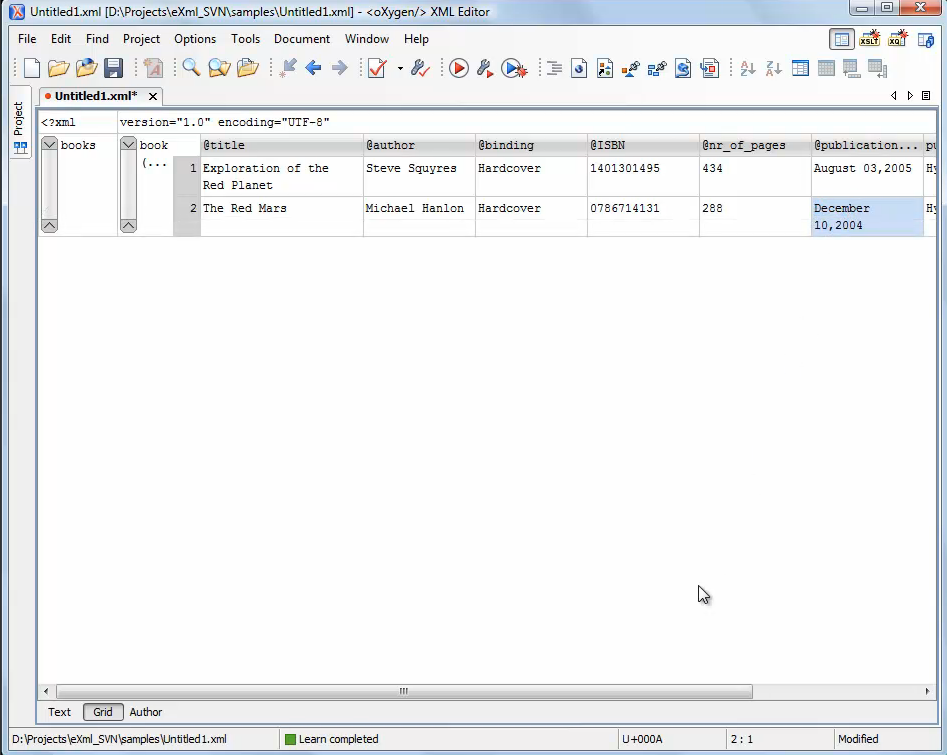
\includegraphics[scale=0.5]{images/analyse-oxygen1.png}
      \caption[Maquette d'interface]{Maquette qsdqdsqsdd'interface.}
\end{figure}


\vfill
\clearpage

\begin{figure}[h!]
\begin{minipage}[b]{\linewidth}
\centering 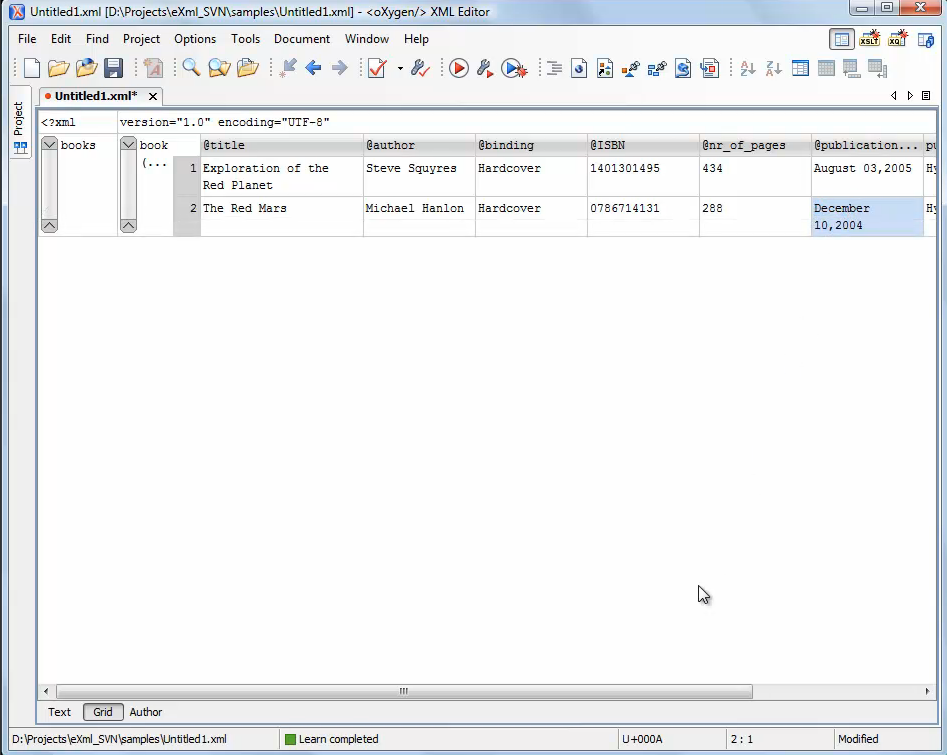
\includegraphics[scale=0.5]{images/analyse-oxygen1.png}
\caption{Exemple de vue avec Oxygen}
\label{oxygen}
\end{minipage}
\end{figure}


\section{Analyse des besoins fonctionnels}
L'objectif du projet est de développer un éditeur XML multi-vues avec différentes fonctionnalités.
\paragraph{}
Les fonctionnalités liées à un éditeur de texte simple devront être présentes : la possibilité de saisir manuellement au clavier l'intégralité du fichier, la création et la sauvegarde du fichier à manipuler ainsi que l'ouverture d'un fichier déjà existant dans le but de le modifier.
\paragraph{}
Des fonctionnalités d'éditeur de texte avancées seront aussi présentes : coloration syntaxique et indentation automatique du code permettant ainsi une lisibilité claire des fichiers manipulés et une autocomplétion du code écrit permettant un gain de temps au cours de la frappe.
\paragraph{}
Pour finir, l'éditeur proposera des fonctionnalités spécifiques au langage XML : validation syntaxique du fichier, vue arborescente du fichier XML avec possibilité de modification des données via cette vue et ajout d'un schéma sur lequel la validation se basera.
\paragraph{}	
La figure \ref{maquette_interface} expose la maquette d'interface de l'éditeur avec chacune des parties annoncées : à gauche la vue arborescente affichant chaque nœud de l'arbre formé par les données, à droite l'éditeur de texte avec toutes ses fonctionnalités associées et en haut la barre d'outils avec la gestion de fichiers (nouveau fichier, ouvrir, sauvegarder) ainsi que la gestion du schéma.

\begin{figure}[h!]
\begin{minipage}[b]{\linewidth}
\centering 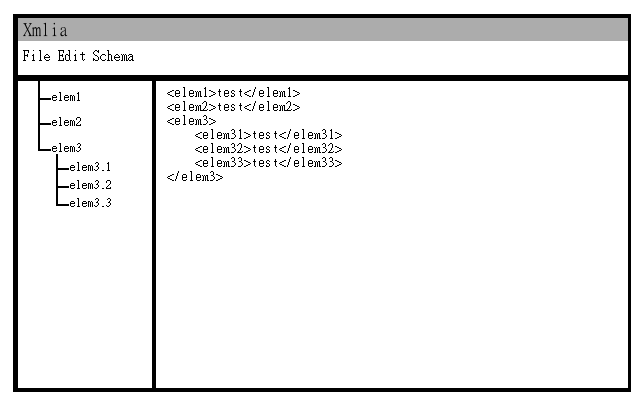
\includegraphics[scale=0.5]{images/analyse-maquette.png}
\caption{Maquette d'interface}
\label{maquette_interface}
\end{minipage}
\end{figure}
	
\section{Analyse des besoins non fonctionnels}
\subsection{Spécifications techniques}
Le programme devra permettre de créer des fichiers XML structurés avec un respect des normes de balisage et, s'il est défini, du schéma de données. De plus, les données saisies ou modifiées à l'aide de l'éditeur doivent rester exploitables, sans corruption du fichier original. Pour terminer, l'éditeur aura à répondre dans des durées acceptables et de manière stable, dans la mesure où la taille et la complexité des données restent raisonnables.
		
\subsection{Contraintes ergonomiques}
Le logiciel devra être suffisamment simple pour qu'un utilisateur connaissant déjà le fonctionnement du XML puisse l'utiliser sans être bloqué par une courbe d'apprentissage trop élevée. On utilisera pour cela des icônes claires et des textes explicatifs.
\paragraph{}
Un utilisateur avancé pourra augmenter sa productivité en utilisant les raccourcis clavier disponibles et pourra gagner de temps en réduisant les transitions souris/clavier.

\chapter{Rapport d'activité}

\section{Organisation du travail}
        
\subsection{Commmunication}

        La communication s'est au départ faite au travers de réunions hebdomadaires au cours desquelles le cahier des charges a été défini auprès de M. Meynard.
        
        Une fois le cahier des charges défini et rendu, le but suivant a été de déterminer quel langage et quel bibliothèque d'affichage graphique sélectionner pour le projet et ainsi être conscient des avantages et des limites des éléments choisis.
        
        Ensuite, l'objectif suivant a été de définir une maquette du logiciel afin de savoir quelles seront les fonctionnalités retenues, la manière de les exploiter et quel organisation visuelle du logiciel sera retenue. C'est ainsi qu'a été définie la maquette qui comporte une interface simple avec une barre d'outils, une vue principale sur le côté droit avec le système d'éditeur de texte, une vue secondaire sur la gauche avec la vue arborescente du modèle XML du fichier présenté par l'utilisateur et enfin la fenêtre de log associé au différents messages liés à l'utilisation de l'éditeur, par exemple, des erreurs de schéma.
        
        Il fallait enfin définir l'organisation du travail au sein du groupe avec des tâches définies et mettre un place un plan de travail, c'est donc Stéphane WOUTERS, le chef du projet, qui a mis en place le gestionnaire de projet, a décidé des moyens de communication et qui a défini le premier objectif de développement : l'apprentissage de la librairie.
        
        Puis la phase d'apprentissage et de développement commença, il fallait alors découvrir et apprendre le framework utilisé, et commencer à développer pour le projet, la communication s'est donc faite au travers de messages sur Google Hangouts, de mails, de commentaires via le gestionnaire de projet et de communication orale dans une salle informatique de la faculté.
        
        \subsection{Répartition des tâches}

\section{Outils de développement}

\subsection{Langage et bibliothèques}

Nous avons utilisé Qt comme bibliothèque d'interface graphique. 

\subsection{IDE}
Nous avons naturellement utilisé Qt Creator comme IDE, c'est en effet l'IDE 

        \subsection{Gestionnaire de projet}
        Le gestionnaire de projet utilisé est Bitbucket, un site Internet d'hébergement mutualisé supportant des projets utilisant Mercurial ou Git comme gestionnaire de versions. Dans le cas de Xmlia, Git a été retenu et utilisé.
        
        Git a ici permis de gérer les accès et les mises à jour différents fichiers du projet, qu'ils soient du code ou du texte brut, comme par exemple pour le rapport du projet. Son utilité aura donc été de permettre une gestion des fichiers de manière formelle, avec des gestions de conflits de versions de fichier, par exemple avec un système de gestion de fichiers basique comme un FTP, si deux développeurs travaillent en accès concurrentiel sur le même fichier, chacun aura alors sa version du fichier et au moment de renvoyer le travail effectué sur le serveur FTP, un conflit de version surviendra, c'est pour cela que Git est utile en mettant en place des barrières empêchant ce genre de problèmes et proposant des solutions pour, par exemple, réunir les deux fichiers et qu'un développeur s'occupe de "merge" ces deux fichiers en un seul qui aura alors le code des deux développeurs. Un dernier point important à aborder est le fait qu'un envoi de code sur le serveur peut être annulé si par exemple une erreur d'utilisation de Git a été faite et que des fichiers auraient alors été modifiés rendant le projet non fonctionnel.
       
       Bitbucket est un service accessible depuis une page Web permettant la gestion de projet Git. Le service propose donc un serveur Git fonctionnel avec une interface Web très performante. Cette interface permet de gérer tous les projets auxquels on est rattaché, créer de nouveaux projets et gérer les droits liés à ces projets. Un nouveau projet a donc été créé sur le site au travers de l'interface puis les droits de modification du projet ont été données aux autres membres du groupe projet qui ont alors pu commencer à utiliser le Git du projet. Ajouté à cela, Bitbucket liste l'intégralité des différentes opérations effectuées sur le Git permettant un regard global et rapide sur toutes les réalisations et offre aux différents membres du groupe la possibilité d'écrire des commentaires sur chaque opération, les membres seront donc notifiés par e-mail de ce changement, ce qui aura été un moyen de communication très présent au cours de la phase de développement. De plus, une fonctionnalité très importante de Bitbucket pour la gestion de projets est le système de tickets qui est intégré à l'interface Web où chaque membre peut ajouter soit une tâche à effectuer ou un bug à corriger et l'affecter à un autre membre, cela permet alors d'avoir une communication plus claire et concise, donnant un regard des autres membres sur les tâches effectuées par le groupe, aussi en leur donnant la possibilité de commenter ces tickets et d'ajouter des informations nécessaires à la réalisation de la tâche, donnant alors un point de vue global sur l'avancement du projet.
       
       Par exemple, l'illustration suivante montre un ticket concernant une fonction à coder avec une description précise et des commentaires afin de mettre l'accent sur le sens de la tâche à réaliser, afin d'avoir une compréhension plus claire du problème.
       
\begin{figure}[H]
      \centering
      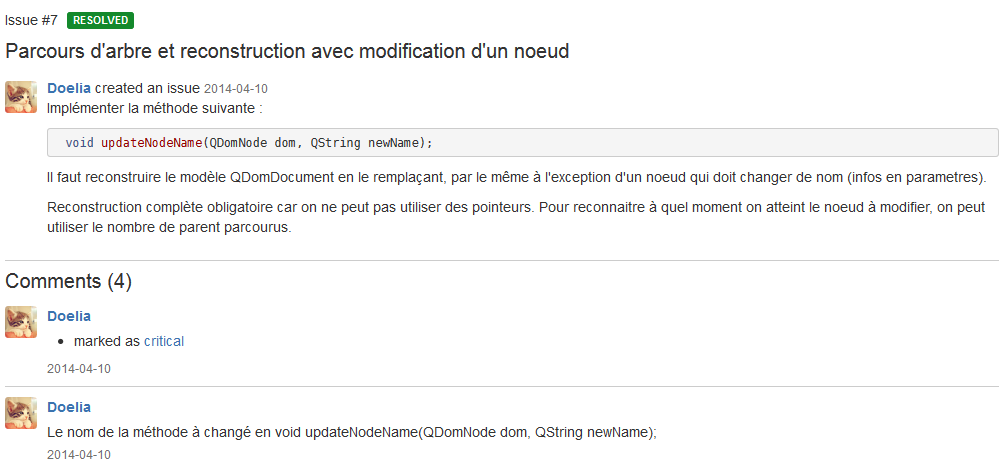
\includegraphics[scale=0.5]{images/bitbucket-exemple-issue.png}
      \caption[Exemple de ticket sur Bitbucket]{Exemple de ticket sur Bitbucket.}
\end{figure}


\chapter{Rapport technique}

\section{Conception}


\section{Architecture de l'application}
\subsection{Le modèle}
\subsection{L'arborescence}

\subsection{L'éditeur de texte}
L'éditeur de texte est décomposé en deux parties, l'éditeur de schéma et d'éditeur XML. Ce sont en réalité des spécialisation de la classe TextEditor.
\subsubsection{La classe TextEditor}
C'est ici que sont toutes les méthodes servant a l'édition du texte en général, telle que l'insertion de texte, l'indentation ou la coloration.
Nous avons fait le choix de représenter les données de l'éditeur de texte simplement par une QString, pas de référence vers la position d'un noeud ou d'information supplémentaire comme sa taille ou la délimitation de son contenu.
Un noeud étant identifé par son chemin depuis la racine, il faut reconstruire l'arborescence XML à partir de la QString. Cela se fait à travers la classe QXmlStreamReader qui s'utilise de la manière suivante :
\lstset{language=C++, inputencoding=utf8}
\begin{lstlisting}
  QXmlStreamReader xml(text->toPlainText());
  while(!xml.atEnd())
  {
    if(xml.isStartElement())
    {
      //traitement
    }
    else if(xml.isEndElement())
    {
      //traitement
    }
  }
\end{lstlisting}
On utilise une structure de pile lors de parcours de l'arborescence. On empile l'indice du sommet lorsque l'on rencontre une balise ouvrante et on dépile lorsque l'on rencontre une balise fermante.
On parvient ainsi à se déplacer et à se repérer dans la QString.

Voici le pseudo code de l'algorithme permettant de parcourir l'arbre pour se rendre sur le noeud désiré.

\begin{verbatim}
//noeud que l'on doit trouver dans la QString
var noeudCible
var pile

//Parseur xml de Qt
var xml

Tant que l'on a pas parcouru tout l'arbre
    Si on rencontre une balise ouvrante
        Si la dernière balise rencontrée est une balise ouvrante
            Empiler 0 dans pile
        Sinon
            //c'est que l'on a atteint le fils suivant
            Incrementer le sommet de la pile de 1
        Fin Si
    Sinon Si on rencontre une balise fermante
        Dépiler pile
    Fin Si
    
    Si noeudCible = pile
        Appeler la fonction qui traitera le noeud
        //on arrête le parcours de l'arbre
        retourner
    Fin Si
   
    Sauvegarder la derière balise renconcrée
    Aller à la balise suivante
Fin Tant Que
\end{verbatim}
 

La quasi totalité des méthodes modifiant le texte le font en le parcourant. Que ce soit l'indentation, l'insertion ou la suppression de noeud ou la validation syntaxique, il faut à chaque fois parcourir l'arbre XML. 
\subsection{Le logger}

\section{Résultat}

\chapter{Manuel d'utilisation}

L'interface de l'éditeur est assez intuitive. Les boutons sont peu nombreux et les fonctionnalités moins utilisées sont dans la barre de menu.
Ce manuel liste la totalité des fonctionnalités du logiciel.

\section{Interaction}

\subsection{Barre de menu}


Les actions disponibles dans la barre de menu sont les suivantes :
\begin{itemize}
\item \emph{File...} : Ouvrir / Sauvegarder / Fermer
\item \emph{Edit...} : Indenter
\item \emph{Schéma...}
	\begin{itemize}
	\item \emph{Load schema file} : Ouvre un schéma et le lie automatiquement au fichier XML.
	\item \emph{Generate schema file} : Génère automatiquement un schéma à partir du fichier XML en utilisant les balises connues.
	\item \emph{Delete schéma} : Supprime la liaison entre le schéma et le fichier XML.
	\end{itemize}
\end{itemize}

\paragraph{}
Les actions Ouvrir, sauvegarder, indenter et valider sont disponibles en accès rapide sur la barre des boutons.

\subsection{Raccourcis}
\begin{itemize}
\item \emph{ctrl + o} : Ouvrir
\item \emph{ctrl + r} : Lancer la validation
\item \emph{ctrl + s} : Enregistrer 
\item \emph{ctrl + shift + s} : Enregistrer sous
\item \emph{ctrl + i} : Indenter automatiquement les lignes sélectionnées
\item \emph{F4} : Switch entre le fichier XML et le schéma
\end{itemize}

\section{Validation}
La validation permet de vérifier si le code XML entré est valide.
Il vérifie que les balises sont correctement formés (pas de balises croisés).
Et si un schéma est associé, le validateur vérifie que le fichier XML est bien en accord avec celui-ci.
En cas d'erreur, le message d'erreur est indiqué dans la console et le numéro de la ligne concernée est surligné en rouge.
Si la validation s'exécute correctement, la vue arborescence est générée.

\section{Vue arborescente}
Sur la vue arborescence il est possible de renommer un noeud (double clic), supprimer un noeud (clic droit / Supprimer), ou déplacer un noeud (glisser/déposer).
Lors d'une modification, la vue de l'éditeur de texte est automatiquement mise à jour.

\section{A propos du schéma}
L'association d'un schéma est une option du logiciel mais il n'est pas obligatoire de lier un schéma pour travailler un fichier XML.
Quand un schéma est ouvert, il est "lié" au fichier XML. La balise de lien vers le schéma est automatiquement ajoutée dans le fichier XML
et un enregistrement provoque la sauvegarde des deux fichiers (xml et schéma).
Lors de l'ouverture d'un fichier XML, le schéma est automatiquement ouvert si un chemin vers celui-ci est indiqué dans le XML.

\section{Fonctions du logiciel}


\begin{figure}[h!]
\noindent\makebox[\textwidth]{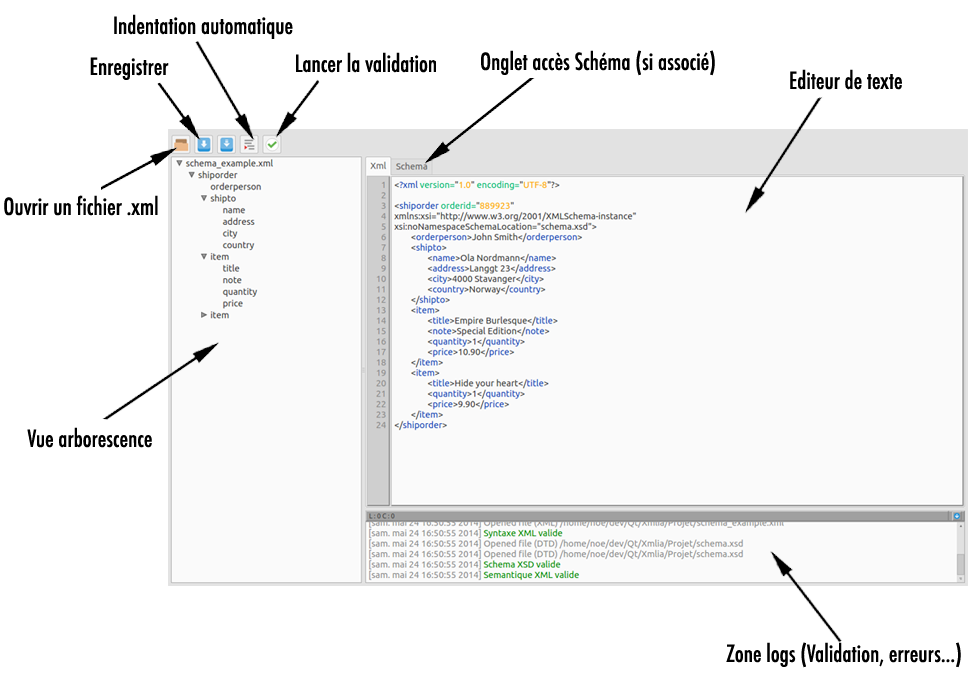
\includegraphics[width=450pt]{images/help1.png}}
\caption{Différentes sections du logiciel}
\end{figure}

\chapter{Perspectives et conclusions}
	\section{Perspectives}
	
	\section{Conclusions}
\listoffigures

\appendix

\end{document}

